% !TeX spellcheck = de_DE
\documentclass{alex_gp}

\name{Alexander Helbok}
\course{Grundpraktikum}
\hwnumber{6}
\spacing{}


\begin{document}
\renewcommand{\labelenumi}{\alph{enumi})}


\begin{mybox}{Stärke und Inklination des Erdmagnetfeldes}
	Ziel dieses Versuches ist es, sowohl den Betrag, als auch die Ausrichtung des Erdmagnetfeldes in Innsbruck zu bestimmen. Dafür wird der Magnetsensor  des IOLab verwendet. Diese muss zuerst kalibriert werden. 
	
	Der Magnetsensor misst das Magnetfeld ich die drei (kartesischen) Raumrichtungen. Um die Berechnung des Magnitude und Inklination des Magnetfeldes zu vereinfachen, drehen wir unser Koordinatensystem (das IOLab) so, dass der Sensor im Rahmen der Unsicherheit einen Wert von 0 in eine Raumrichtung ausgibt. In unserem Fall war das die y-Komponente, welche minimiert wurde. Dann ergibt sich nämlich für den Gesamtbetrag des Erdmagnetfeldes 
	\begin{equation}\label{eqn:mag1}
		|\vec{B}| = \sqrt{B_x^2 + B_z^2}
	\end{equation}
	und für den Inklinationswinkel
	\begin{equation}\label{eqn:theta1}
		\theta = \arctan(\tfrac{B_z}{B_x})
	\end{equation}
	
	Die Messung wurde am Boden durchgeführt durchgeführt und lief etwas über \( 30 \unit{s} \). Die gewonnen Daten sind in \autoref{fig:Bmean} dargestellt. Es wurde für jede Komponente der Mittelwert gebildet und der Fehler auf die Standardabweichung gesetzt, da dann (per Definition) zwei drittel der Daten innerhalb des \( 1\sigma \) Intervalls liegen. 
	
	\begin{figure}[H]	
		\centering
		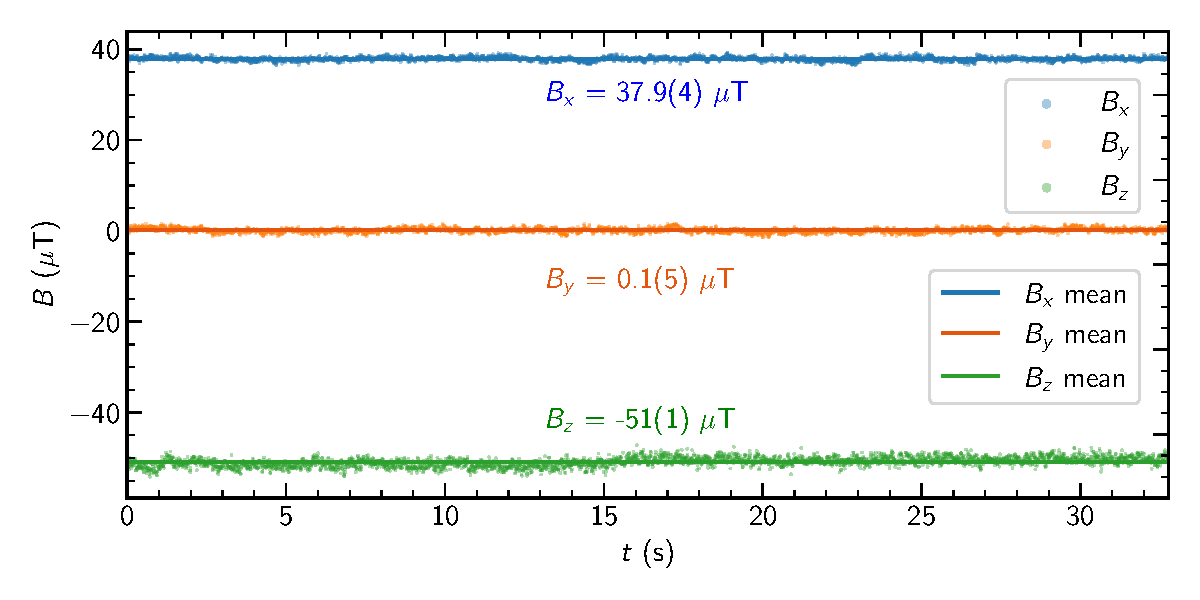
\includegraphics[width=\textwidth]{Versuch6_1}
		\caption{Das gemessene Magnetfeld in die drei kartesischen Raumrichtungen farblich unterscheidbar auf die Zeit aufgetragen. Der Mittelwert der Daten wird als durchgezogene Linie dargestellt.}
		\label{fig:Bmean}
	\end{figure}
	
	Man erhält für die drei kartesischen Komponenten des Erdmagnetfeldes
	\begin{equation}\label{eqn:Bxyz}
		B_x = 37.9(4) \unit{\micro T} \qquad B_y = 0.1(5) \unit{\micro T} \qquad B_z = -50.9(1.0) \unit{\micro T}
	\end{equation}

	Daraus lässt sich jetzt mit \autoref{eqn:mag1} und \autoref{eqn:theta1} die Stärke und Inklination des Erdmagnetfeldes berechnen und man erhält folgende Werte
	\begin{equation}\label{eqn:results}
		|\vec{B}| = 63.4(9) \unit{\micro T} \hspace{3cm} \theta = \ang{53.3(6)}
	\end{equation}
	
	Vergleicht man diese Werte mit Literaturwerten \footnotemark[1]
	\begin{equation}\label{key}
		|\vec{B}| = 48.40(15) \unit{\micro T} \hspace{3cm} \theta = \ang{63.5(2)}
	\end{equation}
	erkennt man, dass unsere gemessenen Werte signifikant abweichen. Das liegt wahrscheinlich daran, dass am Versuchsort eine Vielzahl an metallische Objekte vorhanden waren, die Magnetfelder beeinflussen oder sogar selber erzeugen. Der Versuch wurde nämlich in einem Gebäude aus Stahlbeton durchgeführt, in einem Raum voller Elektronik und oberhalb Labore, in welchen Experimente mit elektrischen und Magnetische Felder durchgeführt werden. Es kommt daher zu systematischen Abweichungen, die verringert werden können, indem man die Messung fern von metallischen Objekten wiederholt.

	\footnotetext[1]{https://www.ngdc.noaa.gov/geomag/calculators/magcalc.shtml\#igrfwmm}
\end{mybox}

\begin{mybox}{Elektromotor}
	
\end{mybox}

\begin{mybox}{Strom durch Leiter}

\end{mybox}


\end{document}